\chapter{JVM Bytecode}
\label{chap:JVM_bytecode}
This chapter will talk about the "Code Generation" part of the figure
\ref{fig:java_pipel}. Optimization will come latter as we want first to have
something that runs, than to optimize it. In the end optimization is just a way
to generate fast machine code, so these to concepts are tangled together.
Besides, in the JVM pipeline, optimization does not matter as much. Going from
semantic analysis to bytecode generation which is executed in the virtual
machine, it's then the job of the VM (JIT in case of Java) to optimize the code.

\section{Code Generation}
As the course name suggests "Languages and Translators" compilers are a little
bit like translators, they take the original source code and translate it into:
\begin{itemize}
    \item Machine code (Intel x86, LLVM, etc.)
    \begin{itemize}
        \item Need of manual optimization
        \item Very large instruction set (x86 > 1000)
        \item It is the lowest level but also more work(but the fastest!)
    \end{itemize}
    \item Byte code (higher level and smaller JVM ~ 200)
    \item Source code (e.g Java poet translate our language in an other one)
    (Simplest but more limited, slowest (as we do duplicate work, all the pipeline is run twice))
\end{itemize}

\subsection{Why JVM?}
\begin{itemize}
    \item JVM byte code have a good effort/result trade off
    \item Built-in in garbage collector (not good if you want your own)
    \item Built-in JIT compiler
    \begin{itemize}
        \item No need for bytecode optimization
        \item Per-CPU instruction selection (always select the best instruction
        for the CPU that runs the code!)
    \end{itemize}
    \item Built-in polymorphism
    \item Ecosystem (call to and from Java)
    \item Can map line to numbers to instructions
    \item Portable (does not need to have different generation for Unix/Mac/Windows, etc)!
    \item Can be package with JVM, jlink, jvm, GraalVM, etc. in order to allow
    the client to not install many libraries.
\end{itemize}
\section{Bytecode}
See slide 6 in order to have an example. The bytecode file starts with some
metadata: name of the class, java version, ACC\_PUBLIC (method is public),
ACC\_SUPER is historical than we have constant pool (\#21 and \#2) which tell the
classes but also the number of methods, attributes, interface, etc.
\subsection{Constant pool}
\theoremstyle{definition}
\begin{definition}[Constant pool]
    Place where constant data are stored. It is a mapping from key to value.
    It use Strings, including:
    \begin{itemize}
        \item string literals used in programs
        \item (full) class names, fields and methods names
        \item methods and fields (type) descriptors
    \end{itemize}
    but also big integer and floating-point number and dynamically computer
    constant (for optimization).
\end{definition}
i.e: \#1 = Methodref \#2.\#3 which point to 2 and 3 \#3 NameAndType which point to
<init> and :()V (parameters that returns void). See other examples on slide 7.
See other examples on slides 8-9. 

\section{JVM Bytecode Instructions}
Now we will see the 200 JVM Bytecode instructions.
\subsection{Execution Model/Data}
Different data storage are used in the JVM bytecode:
\begin{itemize}
    \item Locals (parameters, local variables)
    \item Stack (no register)
    \item Object with fields
    \item Static fields
\end{itemize}
Methods:
\begin{itemize}
    \item Static methods (always know the code that will be executed)
    \item Virtual methods (need to look at which class and thus, to which implementation to call)
\end{itemize}

Note that, the JVM deals with 32 bits values however we know that double and
long are 64 bits each: both occupy two slots (stack of size 2). Shorts and bit
are extended to 32 bits.

\subsection{Instructions}
\theoremstyle{definition}
\begin{definition}[JVM Instruction]
    Each instruction has a name and optionally some immediate byte operands
    referencing the constant pool (most frequent ), offsets (for jumps) or
    immediate (small) integer values (short maximum)). They can modify the stack
    (push, pop, reorder, etc.) Coded as one-byte opcode, maximum 256
    instructions are possible. There is still a possibility to extend them with
    variable length opcode (not needed actually, the opcode 256 is the opcode
    for variable length and the second byte would give 256 more possibilities.)
\end{definition}

\subsubsection{Load/Store}
    \theoremstyle{definition}
    \begin{definition}[Push/Load]
        Push(load) variables on the stack, store value in variables.
        Pattern: (A/F/D/I/L)(LOAD/STORE)[\_0\_1\_2\_3].
        \begin{itemize}
            \item Address (Object), Float, Double, Integer, Long
            \item Numbers are optional and mean load/store from/to variable
            number 0, 1, ... as it it optinal we could also specify the variable
            index as an operand
            \item e.g: ALOAD (load an object from a variable), ISTORE\_0 (store an integer in variable 0)
            \item Why do we have 0/1/2/3? Why not always the generic method?
            Well, 0,1,2,3 only take one byte while the generic one need one byte
            for the instruction and 1 for the variable index. As we want the
            bytecode to be as small as possible (less read/write, less cache
            write, etc.). 0, 1, 2, 3 where just encoded because they are the
            most used once and developer of the JVM had space to encode them.
        \end{itemize}
        There are 50 of them!
        Simple form: one parameter (one byte) to give the variable index.
    \end{definition}
    \theoremstyle{definition}
    \begin{definition}[IINC]
        Parameters: two bytes. Adds the parameter value to the integer variable.
        Often used (like in for loop)
    \end{definition}
    \theoremstyle{definition}
    \begin{definition}[WIDE]
        Modifier of LOAD/STORE/IINC to access a wider range of local variables.
        It uses three bytes of variable space index instead of just one.
        (Preserve the opcode space).
    \end{definition}
\subsubsection{Constants}
    Push constants onto the stack, there are 20 instructions for that.
    \theoremstyle{definition}
    \begin{definition}[ACONST\_NULL]
        Push null onto the stack.
    \end{definition}
    \theoremstyle{definition}
    \begin{definition}[ICONST(\_M1/\_0/\_1/\_2/\_3/\_4/\_5)]
        Push integer -1 / 0 / 1 / 2 / 3 / 4 / 5 onto the stack
    \end{definition}
    \theoremstyle{definition}
    \begin{definition}[FCONST(\_0/\_1/\_2)]
        Push float 0 / 1 / 2 onto the stack.
    \end{definition}
    \theoremstyle{definition}
    \begin{definition}[(L/D)CONST(\_0/\_1)]
        Push long (or double) 0 or 1 onto the stack.
    \end{definition}
    \theoremstyle{definition}
    \begin{definition}[LDC, LDC\_W, LDC2\_W]
        LDC take a pool constant reference and load the constant. LDC\_W also
        take a constant pool reference but take 2 bytes instead of one and
        LDC2\_W is the same but allow us to push two 32bits value (long or
        double).
    \end{definition}
    \theoremstyle{definition}
    \begin{definition}[BIPUSH/SIPUSH]
        BIPUSH push a byte. SIPUSH push a short.
    \end{definition}

    Theoretically LDC[2]\_W would allow us to do everything, but once again,
    encode the most common operation is nice to reduce the executable size.
\subsubsection{Type conversions}
Java has implicit type conversion (1+2L will convert the integer into a long)
\theoremstyle{definition}
\begin{definition}[(I/D/F/L)2(I/D/F/L)]
    No identity conversion, just pop a value and push its conversion onto the stack.
\end{definition}
\theoremstyle{definition}
\begin{definition}[I2(B/C/S)]
    This operation is the truncation of integer to a byte (null the unused bits).
\end{definition}
\subsubsection{Arithmetic/Binary Operations}
Pop two values from the stack and push the result of the operation on the stack.
\theoremstyle{definition}
\begin{definition}[(D/F/I/L)(ADD/DIV/MUL/SUB/NEG/REM)]
    Does the corresponding operation...
\end{definition}
\theoremstyle{definition}
\begin{definition}[(I/L)(AND/OR/SHL/SHR/USHR/XOR)]  
    Only for integer and long we have the classical operation and shift
    left/right(SHL/SHR) but also unsigned shift right(USHR).
\end{definition}
\subsubsection{Stack Manipulation}
\theoremstyle{definition}
\begin{definition}[DUP]
    DUP[2][\_X1/\_X2]. Duplicate a value (take a value on the top
    of the stack.) Adding the 2 duplicate 2 values or a double size value. As
    DUP does not push value onto the stack but insert above the top value, X1
    means "skip a variable", so if the stack is value2, value1 (top of the
    stack). It will be value1, value2, value1 (top of the stack here).
    X2 is the same but skip two values then insert the duplicate.
\end{definition}
\theoremstyle{definition}
\begin{definition}[POP]
    POP[2]. Remove the top value. POP2 remove either two values
    or a 2 bytes value. Note that the value is just removed, we cannot do
    anything with it.
\end{definition}
\theoremstyle{definition}
\begin{definition}[SWAP]
    Swap the two top values of the stack. We can notice that there is no SWAP2
    instruction, so how can we remove 2 bytes long value? Just use DUP\_X2 then
    POP.
\end{definition}
\subsubsection{Arrays}
\theoremstyle{definition}
\begin{definition}[(A/F/D/I/L/C/B/S)A(LOAD/STORE)]
    As variable LOAD/STORE from array of a certain type (CHAR/BYTE/SHORT) we
    have these three types as in arrays they are actually stored as bytes.

    LOAD take an arrayref and an index from the top of the stack remove them and
    push the read value onto the stack.
    STORE take an arrayref, an index and a value and write in into the array.

    Note that BALOAD works for both boolean and bytes (in order to avoid
    representing boolean as integer). Why not as boolean as bits? Best guess is
    it save the instruction to retrieve bit while retrieve bytes, thus the best
    guess is that developers are okay to waste a bit of memory to avoid these
    new operations. 
\end{definition}
\theoremstyle{definition}
\begin{definition}[NEWARRAY] [A]NEWARRAY creates an array of primitive ANEWARRAY
    creates an array of object. Both case take a constant pool reference that
    holds type descriptor or a class object for the component type of the
    object. They also read the length of the array and then push the array onto
    the stack.
\end{definition}
\theoremstyle{definition}
\begin{definition}[MULTIANEWARRAY]
    Create a multi dimensional array of objects. As parameters it take the type
    (constant pool reference) and dimensions. On the stack we will push as many
    counts as the dimensions.

    The reason of the always present A is that, in Java even if we create an 2D
    array of integer, we will create an array with component that are pointers
    to integer arrays.
\end{definition}
Note that a 2D array of integer will use ANEWARRAY (of pointers) then fill it
with NEWARRAY (of integers). MULTIANEWARRAY would be used to create 3D array
(using a size of 2) and the last dimension would store array of integers created
with NEWARRAY.
\theoremstyle{definition}
\begin{definition}[ARRAYLENGTH]
    Pop the array from the stack and push its length onto it.
\end{definition}
\subsubsection{Field Access}
\theoremstyle{definition}
\begin{definition}[GETFIELD/PUTFIELD]
    Take a field reference as an immediate parameter (itself consisting of a
    class, field name and field descriptor (type).)

    GETFIELD takes an objectref from the stack and push the field value.
    PUTFIELD takes an objectref and a value from the stack and assign them.
\end{definition}
\theoremstyle{definition}
\begin{definition}[GETSTATIC/PUTSTATIC]
    Same as the previous but for static fields (no objectef needed.)
\end{definition}

\subsubsection{Comparisons}
Comparisons are not implemented like binary/arithmetic operations in order to
save space. Besides, CPUs architectures like Intel x86 already have these
operation with the same definition as Java. Also, they have separated integers
(because much more used but very very frequent on control flow jump).
\theoremstyle{definition}
\begin{definition}[(D/F)CMP(G/L)]
    D and F are for Double and Float, take two values and push the result onto
    the stack. Let's assume A and B have been taken from the stack: $A>B
    \rightarrow 1$, $A<B \rightarrow -1$, $A==B \rightarrow 0$

    G and L are used to deal with NaN values if the instruction contains G 1
    will be push onto the stack, if it contains L it will be -1.
\end{definition}
\theoremstyle{definition}
\begin{definition}[LCMP]
    Exactly the same but for long.
\end{definition}
\theoremstyle{definition}
\begin{definition}[INSTANCEOF]
    Take a class reference as an immediate parameter and an object from the
    stack. Then push 1 if the object is of the given class, 0 otherwise.
\end{definition}
\theoremstyle{definition}
\begin{definition}[CHECKCAST]
    Same as INSTANCEOF but throws an exception if needed.
\end{definition}

\subsubsection{Jumps and Conditionals}
Parameter for these instructions is always an offset in bytes (2 bytes, 4 for \_W).
It allow to jump backward or forward.
\theoremstyle{definition}
\begin{definition}[GOTO]
    GOTO[\_W]. Unconditional jump. W is for wide that allow the code to jump
    very far away.
\end{definition}
\theoremstyle{definition}
\begin{definition}[IF\_ACMP(EQ/NQ)]
    Two stack operands. Compare the object pointer (the \textit{real} same
    object). It jumps if they are equals otherwise execute the next instruction.
    NE is the opposite.
\end{definition}
\theoremstyle{definition}
\begin{definition}[IF\_ICMP(EQ/NE/GE/GT/LE/LT)]
    Two stack operands. Same but for integers.
\end{definition}
\theoremstyle{definition}
\begin{definition}[IF(EQ/NE/GE/GT/LE/LT)]
    Single stack operand (EQ=0, GT>0, LT<0). Jump if the operand is 0 (EQ) or
    other operand. It is the result of the previous CMP so we can combine them!
\end{definition}
\theoremstyle{definition}
\begin{definition}[IF]
    IF[NON]NULL. Jump if null or not null.
\end{definition}
\subsubsection{Object Creation}
\theoremstyle{definition}
\begin{definition}[NEW]
    Use a class reference as a parameter. It allocate memory for the object
    (does not call the constructor!). In order to call the constructor we have
    to call a special instruction which is INVOKESPECIAL <init> and the bytecode
    verifier checks that a constructor is called.
\end{definition}
\subsubsection{Method Invocation}
Parameter is always the method reference (class, name, method descriptor (type)).
All methods invocation instruction have a reference as immediate parameter.
\theoremstyle{definition}
\begin{definition}[INVOKESTATIC]
    Static methods, not used with "this" on the stack. We always know the code
    that will be executed!
\end{definition}
\theoremstyle{definition}
\begin{definition}[INVOKEVIRTUAL]
    Classical methods calls, using "this" on the stack. It get the object class
    and get the method implementation from its method table (all methods a class
    can use also the methods from the superclass even if they are not
    override). The specific code is not known at the compilation time (can
    change at each call!)
\end{definition}
\theoremstyle{definition}
\begin{definition}[INVOKEINTERFACE]
    Same as INVOKEVIRTUAL but for interface methods but the lookup is a bit more
    complex because we can only inherit from one class but we can implement many
    interfaces.
\end{definition}
\theoremstyle{definition}
\begin{definition}[INVOKESPECIAL]
    Static linking using "this" pointer. Also used for private methods (cannot
    be overriden it is always the same class), constructors (always know which
    class to look in) and super methods (when we do a call, the compiler know
    the type of the "this" object thanks to that it can find the first ancestor
    class that implement the method!).
\end{definition}
\theoremstyle{definition}
\begin{definition}[INVOKEDYNAMIC]
    It is useful to implement dynamic languages. Basically it is a wormhole
    instruction. The first time it is called it goes to a bootstrap method that
    returns a CallSite (need to be implemented!). Once it is done, the
    instruction is patch (does not go to the bootstrap but directly to the
    CallSite). Note that it then can be optimized like any other function call.
    If we save the CallSite object we can change the target of the target method!

    Allowing that is very useful for polymorphic inline caches (always use a
    method tailored to the types that have actually been seen (+ check if the
    values are supported.)). 
\end{definition}

\subsubsection{Misc Instruction}
\theoremstyle{definition}
\begin{definition}[RETURN]
    [A/F/D/I/L]RETURN returns void if no prefix otherwise returns the value.
\end{definition}
\theoremstyle{definition}
\begin{definition}[ATHROW]
    Throw exception.
\end{definition}
\theoremstyle{definition}
\begin{definition}[MONITOR(ENTER/EXIT)]
    Enter and exit monitor (kind of mutex)
\end{definition}
\theoremstyle{definition}
\begin{definition}[NOP]
    Does nothing:
\end{definition}
\theoremstyle{definition}
\begin{definition}[LOOKUPSWITCH/TABLESWITCH]
    Use to optimize the switch statement!
\end{definition}

\section{JIT Register Allocation}
Many lower lover instructions map easily to underlying machine code however most
CPU use registers (register (small but very fast), L1, L2 caches or RAM (big but
really slow)). Caching happens automatically but not in registers! They must be
assigned manually. We cannot map the JVM stack as it would be too expensive so
we have to decide what we can put in the different register (as a lot of machine
code instruction must use registers). it is done by using a register allocation
algorithm.

\section{Differences with Java}
Even if the JVM was made for Java the have some differences:
\begin{itemize}
    \item Generic type does not exists in JVM (they mostly exists in the
    semantic part). Generic types are not reified (no object for it). Still C\#
    have reified generics or we could create a language with generic types using
    the JVM.
    \item No checked exceptions : all exceptions act like the RunTimeException
    in the JVM.
\end{itemize}
These are the main two differences between JVM and Java.

\section{Loading and Verification}
Class files are loaded into the JVM when required (first time the class is being
referred). The JVM use the name to locate the class in the class path. When the
class file is loaded the bytecode is verified (constructor called, final
variables are no rewritten, etc.). A very important verification is the
Typestate: any instruction reachable through multiple paths (first instruction
after an if-else, indeed we could have been by the if or the else part, if one
part push a value on the stack but not the other we have a problem!) must be
reached with the stack in the same state (size and types).
\subsection{Typestate}
    \theoremstyle{definition}
    \begin{definition}[name]
        Any instruction reachable through multiple paths (first instruction
after an if-else, indeed we could have been by the if or the else part, if one
part push a value on the stack but not the other we have a problem!) must be
reached with the stack in the same state (size and types).
    \end{definition}

    Java knows the type of every local and every slot on the stack (the machine
    code does not know that!). 

    It is not possible to iterate an array to copy it on the stack because the
    typestate would be different depending of the array type.

    The stack can't overflow if you don't recurse.

\section{Summary}
    JVM performs stack-based computation, use stacks + locals + constant pool +
    fields. Build in GC (cost of the memory control), built-in JIT complier! JVM
    Bytecode has a low level stack operations, jumps. It can transfers between
    stack and locals, fields, constant pool. It has highly-abstracted
    polymorphic method calls.

\section{Generating Bytecode with ASM}
ASM is a low level library and comprehensive to generate Bytecode, other
libraries exists (BCEL, Javassists, etc.). Some interesting libraries are
ByteBuddy or CGLIB which are focused on higher level patterns (dynamic proxy) it
is a class that implement an interface automatically typically delegating the
methods implementation while running code before or after the code
(verification, log, etc.).

The advantage of ASM is that it handle the constant pool, takes care of the
stack and space, manage jumps.  

If we want to use ASM, we can use javap to reverse engineer to know what the
Java compiler would done, read the JavaDoc, manual, Wikipedia page, etc.

\subsection{Notations}
\subsubsection{Field descriptors}
Describe the value of type. We only need to define them when we define or access
a field.
Here is the table of fields descriptors:
\begin{figure}[H]
     \centering
     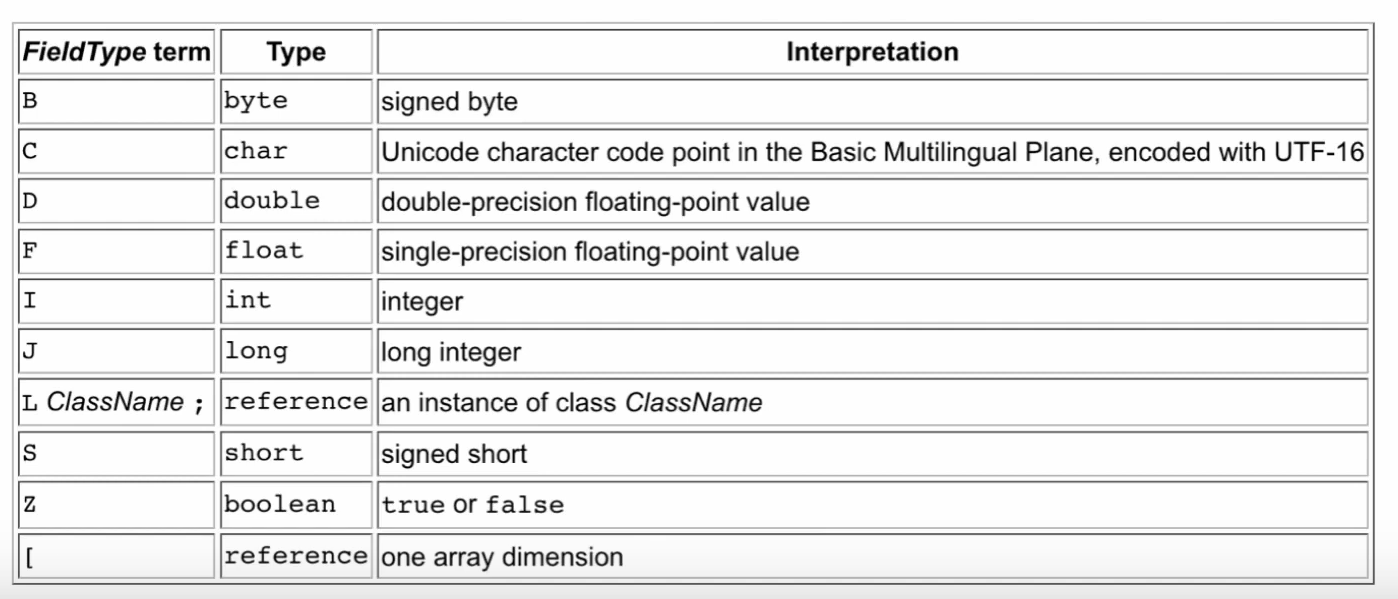
\includegraphics[scale=0.4]{fieldDescriptors}
     \caption{Fields descriptors table}
     \label{fig:field_descriptors}
\end{figure}
Notice that there are some "traps" B is for Byte so Boolean are Z. Long is noted
as J. Note that class are noted L Classname; so either we read an single letter
or a semi colon and we know we have to look the the next two inputs. In order to
describe an array we only need the bracket [ then the type, i.e: [I or [[I dor a
2D int array. V for void type is not needed here as it is a method descriptor
and we're looking at field descriptors here.
\subsubsection{Method descriptor}
Here is the syntax (<param1 field desc><param2 field desc>...)<return field
desc>. Fields descriptors for the parameters, then for the return type.The only
syntax here is the (), we don't need to separate them as we always know how much
we need to read!

\subsubsection{Slash-separated class name}
References to classes are done like that: java/util/String (probably for
historical reasons linked to how it is stored in the disk). These name are unique
Let's imagine a "tricky" example:
\begin{lstlisting}[language=Java]
    package pkg;
    class A {
        static class X{...}
        ...
    }
    package pkg;
    class B extends A{...}
\end{lstlisting}
We could imagine two class name: pkg/A\$X and pkg/B\$X however, only the first
one is valid!